\chapter{Традиционные методы компьютерного зрения}

Компьютерное зрение (иначе техническое зрение) — теория и технология создания машин, которые могут производить обнаружение, отслеживание и классификацию объектов.

Цель компьютерного зрения заключается в формировании полезных выводов относительно объектов и сцен реального мира на основе анализа изображений, полученных с помощью датчиков \cite{computervision}.

Принцип работы традиционных методов компьютерного зрения заключается в извлечении векторов объектов из изображений для их дальнейшей классификации \cite{comparedeep}.

\section{Метод опорных векторов}

Метод опорных векторов (англ. support vector machine, SVM) — один из наиболее популярных методов обучения, который применяется для решения задач классификации и регрессии. Основная идея метода заключается в построении гиперплоскости, разделяющей объекты выборки оптимальным способом.

Алгоритм работает в предположении, что чем больше расстояние (зазор) между разделяющей гиперплоскостью и объектами разделяемых классов, тем меньше будет средняя ошибка классификатора.

Применение метода опорных векторов в распознавании изображений:
\begin{itemize}
	\item Рассматриваем изображение как массив пикселей, если размер изображения 200 X 200, то размер массива будет 200 X 200 X 3, где первые 200 — ширина, а вторые 200 — высота, а затем 3 по значению канала RGB. Значения в массиве будут находиться в диапазоне от 0 до 255, что описывает интенсивность пикселя в каждой точке.
	\item Набор образов изображений загружается для обучения. Сначала преобразует все изображения в опеределённый формат, а затем сглаживает все изображения, в результате чего получается массив n-меры чисел для каждого изображения. Эти массивы используются как 1 точка в n-мерном пространстве.
	\item Построить классификатор изображений методом опорных векторов на основе набора изображений для обучения.
\end{itemize}

\captionsetup{justification=centering,singlelinecheck=off}
\begin{figure}[h!]
	\centering
	%\begin{center}
		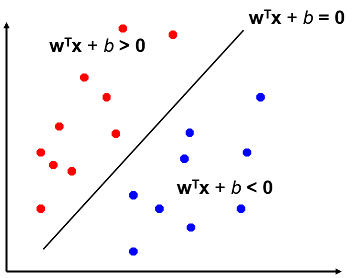
\includegraphics[pages=-, scale=0.9]{img/svm.png}
		\caption{Метод опорных векторов}  
	%\end{center}
\end{figure}

\begin{itemize}
\item Преимущества метода
	\begin{itemize}
	\item Хорошо работает с пространством признаков большого размера;
	\item Хорошо работает с данными небольшого объема;
	\item Метод находит разделяющую полосу максимальной ширины, что позволяет в дальнейшем осуществлять более уверенную классификацию.
	\end{itemize}

\item Недостатки метода
	\begin{itemize}
	\item Долгое время обучения (для больших наборов данных);
	\item Неустойчивость к шуму: выбросы в исходных данных становятся опорными объектами-нарушителями и напрямую влияют на построение разделяющей гиперплоскости.
	\end{itemize}
\end{itemize}

\section {Метод k-ближайших соседей}

Метод k-ближайших соседей (k-nearest neighbors) – это простой алгоритм машинного обучения с учителем, который можно использовать для решения задач классификации и регрессии.

Алгоритм K-NN сохраняет все доступные данные и классифицирует новую точку данных на основе сходства. Это означает, что когда появляются новые данные, их можно легко классифицировать по категории наборов с помощью алгоритма K-NN.

Согласно принципу алгоритма KNN, структура классификатора включает в себя 4 параметра: данные для классификации, набор выборочных данных, набор выборочных меток и значение K. Затем вычислить расстояние между новыми данными и выборочными данными, упорядочить расстояния от наименьшего к наибольшему, возьмите первые K ближайших данных. Наиболее часто встречающаяся метка может быть идентифицирована как новая метка данных путем определения количества вхождений каждого введенного типа данных в К первых точках.

\captionsetup{justification=centering,singlelinecheck=off}
\begin{figure}[h!]
	\centering
	%\begin{center}
		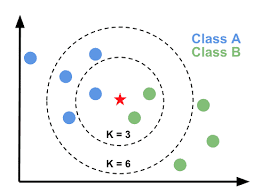
\includegraphics[pages=-, scale=0.9]{img/knn.png}
		\caption{Метод опорных векторов}  
	%\end{center}
\end{figure}

\begin{itemize}
\item Преимущества метода
	\begin{itemize}
	\item Алгоритм прост и легко реализуем.
	\item Не чувствителен к выбросам.
	\item Нет необходимости строить модель, настраивать несколько параметров или делать дополнительные допущения.
	\item Алгоритм универсален. Его можно использовать для обоих типов задач: классификации и регрессии.	
	\end{itemize}

\item Недостатки метода
	\begin{itemize}
	\item Алгоритм работает значительно медленнее при увеличении объема выборки, предикторов или независимых переменных.
	\item Из аргумента выше следуют большие вычислительные затраты во время выполнения.
	\item Всегда нужно определять оптимальное значение k.
	\end{itemize}
\end{itemize}

\section{Вывод}

Таким образом, традиционный подход, использующий методы машинного обучения, имеет недостатки: потребность в данных для процесса обучения, низкая скорость обучения для больших наборов данных и неустойчивость к шуму, однако рассмотренные методы просты и легко реализуемы. В настоящее время интерес к машинному обучению возрастает, поскольку машинное обучение выполняет вычислительную обработку намного эффективнее. Также оно позволяет быстро создавать модели, позволяющие анализировать данные большего размера и сложности и дающие результаты быстрее и точнее. Благодаря своей эффективности и выдающимся преимуществам машинное обучение станет целенаправленным и увлекательным.

